
\subsection{Introduction}
The following section provides technical details on the jammer equipment used in the experiments. The jammers are categorized according to the following scheme:

\begin{table}[H]
\begin{tabular}{|l|l|l|}
\hline \rowcolor[HTML]{C0C0C0} 
\textbf{1st Letter (Norwegian / English)}    & \textbf{1St digit}                             & \textbf{2nd digit}                     \\
\hline
S = Sigarett / Cigarette            & \multirow{5}{*}{Number of antennas}   & \multirow{5}{*}{\# jammer within same category} \\
\cline{1-1}
H = Håndholdt / Handheld            &                                       &                       \\
\cline{1-1}
U = USB / USB stick                 &                                       &                       \\
\cline{1-1}
F = Fastmontert / Permanently installed (Fixed) &                           &                       \\
\cline{1-1}
M = Mobil / Mobile (Car mounted)    &                                       &                       \\
\hline              
\end{tabular}
\end{table}

\textbf{Exempli gratia:}
S1.2, is a cigarette type jammer, that has 1 antenna, and is unit nr.2 in this category.
\\
\\
\textbf{Additional information:}
\begin{itemize}
    \item Each chapter gives an overview of each jammer brought to Jammertest. As far as possible, it
gives information on
    \begin{itemize}
        \item Centre frequency [MHz]
        \item Bandwidth [MHz]
        \item Power Spectral Density (PSD) [dBm/MHz] for the entire bandwidth
        \item Total output power (TX total) [dBm] for the entire bandwidth
        \item CF max [dBm] (maxhold power at the centre frequency)
        \item Sweep rate [$\mu$s] (if applicable)
        \item Modulation
    \end{itemize}
    \item Indicators such as “L1, L2, L5” etc. are used to indicate main bands of attack, used for
convenience to distinguish between jammers' modus operandi
\item 2023 measurements
    \begin{itemize}
        \item Technical details on low power jammers given in this appendix are from uncalibrated
        measurements. They are rough estimates given for both the frequency and time
        domain. Power levels are not correctly displayed on the chart, because of external
        attenuators used during measurements with a signal analyser. There may also have
        been some constraints in the measurement device, causing fast frequency
        components to not be correctly displayed.
    \end{itemize}
    \item 2024 measurements
    \begin{itemize}
        \item Measurements done with a R\&S FSW. All measurements were performed connected
        directly to the jammers' antenna port, with the other antennas disconnected and (if
        applicable) DIP switches for the other antenna ports disabled. Powe levels etc. should
        be as close to reality as possible for output power at the antenna port.
        \item Throughout the measurements, bandwidth is defined as 3 dB from local (identifiable)
        maxima along the maxhold's descent.
        \item TX power is measured within said bandwidth. Note that TX total is measured over the
        entire bandwidth, so that peak output power is not equal to TX total.
    \end{itemize}
\end{itemize}

%% Content starts here


\input{\filsti equipment}


%% Manual content that does not fit the template;
\subsection{Technical details on the meaconing setup 'Porcellum' / 'F1.1'}
The meaconing setup consists of two GNSS antennas 'E1' and 'E2' at two respective locations some
distance from the transmitting antenna. Real live sky signals from the receivers are (after travelling
through long cables) retransmitted with a directional antenna 'E3' pointing towards the community
house in Bleik. The locations of the receiving antennas are outside of the line-of-sight to the
transmitter antenna to avoid a feedback loop. The setup allows for switching between the two
receiving antennas, ramping power and simultaneous transmission of both signals.
\begin{figure}[H]
    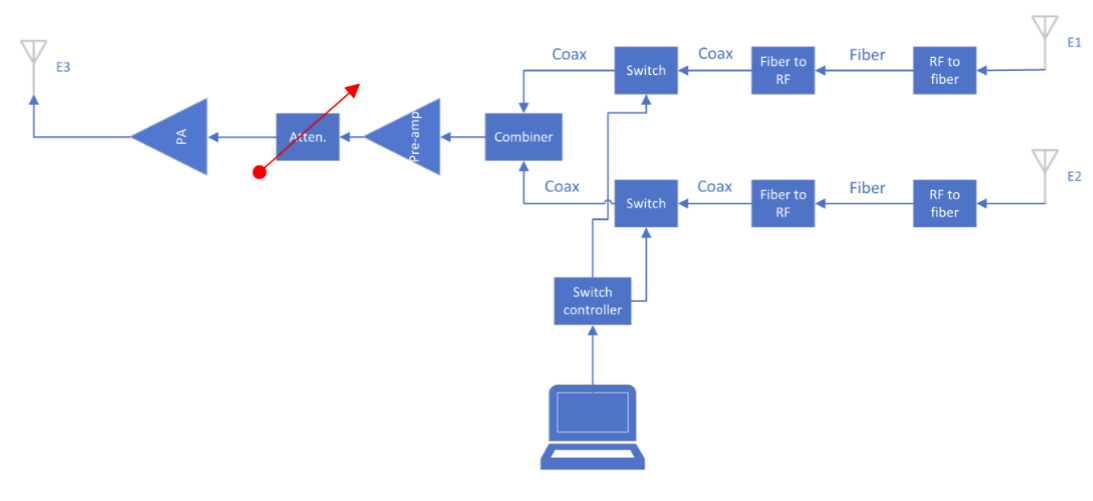
\includegraphics[width=\textwidth]{graphics/appendixG/meaconingSetup.png}
    \caption{Diagram of the meaconing setup}
\end{figure}

\subsection{Technical details on the high-power jammer 'Porcus Maior'/ 'F8.1'}
The high-power jammer provides jamming signals with up to 50 W EIRP simultaneously on eight GNSS
bands, where the maximum available power depends on the signal modulations. Figure \ref{fig: F8.1-1 highPowerJammer} is a
block diagram of the high-power jammer that shows how it works in pniciple. The jammer uses two
USRP X410 SDR from Ettus Research as exciters. Each SDR have four output channels covering the
frequency range of 1 MHz to 7.2 GHz, with maximum 400 MHz instantaneous bandwidth. The SDRs
have an internal gain range of 60 dB in 1 dB steps. Each of the exciter output signals are fed to the
corresponding channel of the programmable step-attenuator. The jammer can also utilize other signal
generators. The attenuator has an attenuation range of 95 dB in 0.25 dB steps. The output signal from
the attenuators is then fed to the power amplifiers. The amplifiers connect to eight individual
antennas via a 10 m coax. The antennas are directional helical antennas with right hand circular
polarization (RHCP) and 10 dB gain.

\begin{table}[H]
\begin{tabular}{|c|c|cc|ccc|}
\hline
\caption{Overview of the signal modulations employed by 'Porcus Maior'}
\rowcolor[HTML]{C0C0C0} 
\cellcolor[HTML]{C0C0C0} & \textbf{CW} & \multicolumn{2}{c|}{\cellcolor[HTML]{C0C0C0}\textbf{PRN}} & \multicolumn{3}{c|}{\cellcolor[HTML]{C0C0C0}\textbf{Frequency sweep}} \\ \cline{2-7} 
\rowcolor[HTML]{C0C0C0} 
\multirow{-2}{*}{\cellcolor[HTML]{C0C0C0}\textbf{\begin{tabular}[c]{@{}c@{}}Frequency\\ band name\end{tabular}}} &
  \textbf{\begin{tabular}[c]{@{}c@{}}Frequency\\ (MHz)\end{tabular}} &
  \multicolumn{1}{c|}{\cellcolor[HTML]{C0C0C0}\textbf{\begin{tabular}[c]{@{}c@{}}Center\\ frequency\\ (MHz)\end{tabular}}} &
  \textbf{\begin{tabular}[c]{@{}c@{}}BPSK\\ chiprate\\ (MHz)\end{tabular}} &
  \multicolumn{1}{c|}{\cellcolor[HTML]{C0C0C0}\textbf{\begin{tabular}[c]{@{}c@{}}Center\\ frequency\\ (MHz)\end{tabular}}} &
  \multicolumn{1}{c|}{\cellcolor[HTML]{C0C0C0}\textbf{\begin{tabular}[c]{@{}c@{}}Sweep rates\\ (kHz)\end{tabular}}} &
  \textbf{\begin{tabular}[c]{@{}c@{}}Frequency\\ bandwidth\\ (MHz)\end{tabular}} \\ \hline
L1  & 1575.42  & 1575.42  & 10 & 1575.42  & 1-100 & 20 \\ \hline
L2  & 1227.6   & 1227.6   & 10 & 1227.6   & 1-100 & 20 \\ \hline
L5  & 1176.45  & 1176.45  & 10 & 1176.45  & 1-100 & 20 \\ \hline
G1  & 1602     & 1602     &  5 & 1602     & 1-100 & 10 \\ \hline
G2  & 1246     & 1246     & 10 & 1246     & 1-100 & 20 \\ \hline
E5b & 1207.14  & 1207.14  & 10 & 1207.14  & 1-100 & 20 \\ \hline
E6  & 1278.75  & 1278.75  & 10 & 1278.75  & 1-100 & 20 \\ \hline
B1I & 1561.098 & 1561.098 &  1 & 1561.098 & 1-100 &  2 \\ \hline
\end{tabular}
\caption{Overview of the signal modulations employed by 'Porcus Maior'}
\end{table}

A PC controls the high-power jammer, that is both exciters and the step-attenuators. Software allows
for the jammer to automatically execute individual tests described for the high-power jammer and
supports all jamming signals described therein.
The high-power jammer is connected to Internet and time synchronized using Network Time Protocol
(NTP). After a jamming activity, it can upload the activity log to the central server.

\begin{figure}[H]
    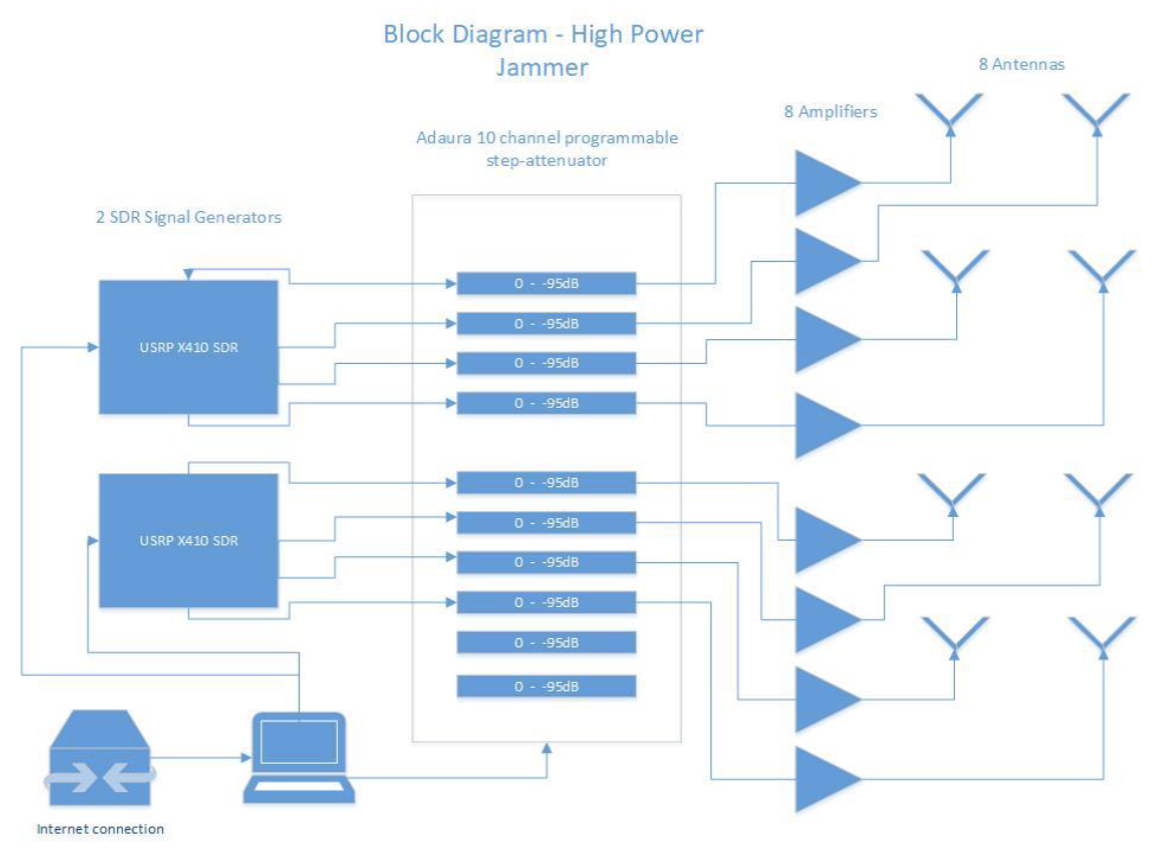
\includegraphics[width=\textwidth]{graphics/appendixG/blockDiagramHighPowerJammer.png}
    \caption{Diagram of the high-power jammer}
    \label{fig: F8.1-1 highPowerJammer}
\end{figure}

\subsection{Technical details on software defined radio mobile SDR spoofer 'F1.2'}
A software defined radio (SDR) of type BladeRF x115 from Nuand is used for the mobile spoofing
tests. The output signal is amplified 45 dB through an AA MCS 800 – 2200MHz amplifier, so that the
maximum total EIRP is about 10 dBm. This signal is transmitted by a dipole antenna on the top of the
vehicle, see \href{https://www.european-antennas.co.uk/media/1900/ds1036-080410.pdf}{ds1036-080410.pdf} (european-antennas.co.uk). \\\\
\begin{figure}[hbt!]
    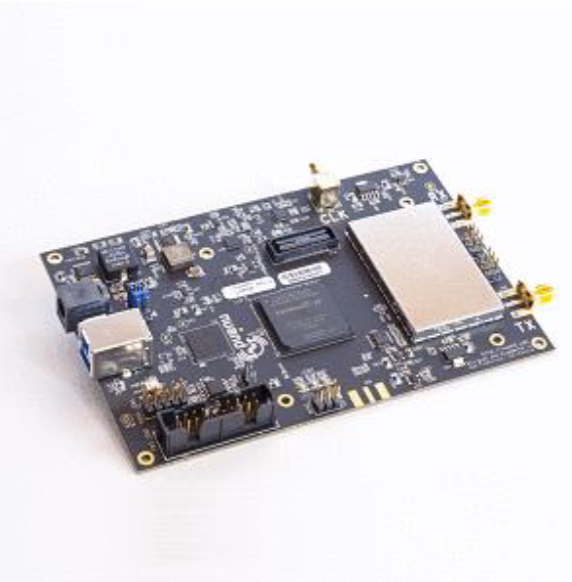
\includegraphics[scale=0.4]{graphics/appendixG/SDR.png}
    \caption{Picture of the SDR without casing}
\end{figure}

The spoofed signals are GPS C/A only and may be combined with Glonass jamming (G1).

\subsection{Technical details on software defined radio mobile SDR spoofer 'Winnie-the-spoof' / 'M1.1'}
Winnie-the-spoof is vehicle based high-power mobile jammer and spoofer that can provide signals up to 50 W EIRP simultaneously between three and six different GNSS bands,
 where the maximum available power depends on the signal modulations. Figure \ref{fig: M1.1-1 Winnie-the-spoof} is a block diagram of the vehicle's equipment. 
 To generate the signals it uses an Orolia GSG-8 simulator with four Dektec DAT-2115B SDR-cards. 
 Each SDR has one output covering the frequency range from 32 MHz to 2.1 GHz, with maximum 72 MHz instantaneous bandwidth. 
 The SDRs have an internal gain range of 60 dB in 1 dB steps. Final power output is controlled using step-attenuators and high power amplifiers. 
 Each amplifier is connected to its own antenna via a 6m coax cable. 
 The antennas are directional helical antennas with right hand circular polarization (RHCP) and 10 dB gain, 
 vertical horn antennas (13dB gain) or an isotropic vertical radiator (0dB gain) for the spoofing, depending on the scenario. 
 The system can simultaneously jam and spoof most combinations of bands, limited only by the intermodulation of the final amplifiers.

\begin{figure}[H]
    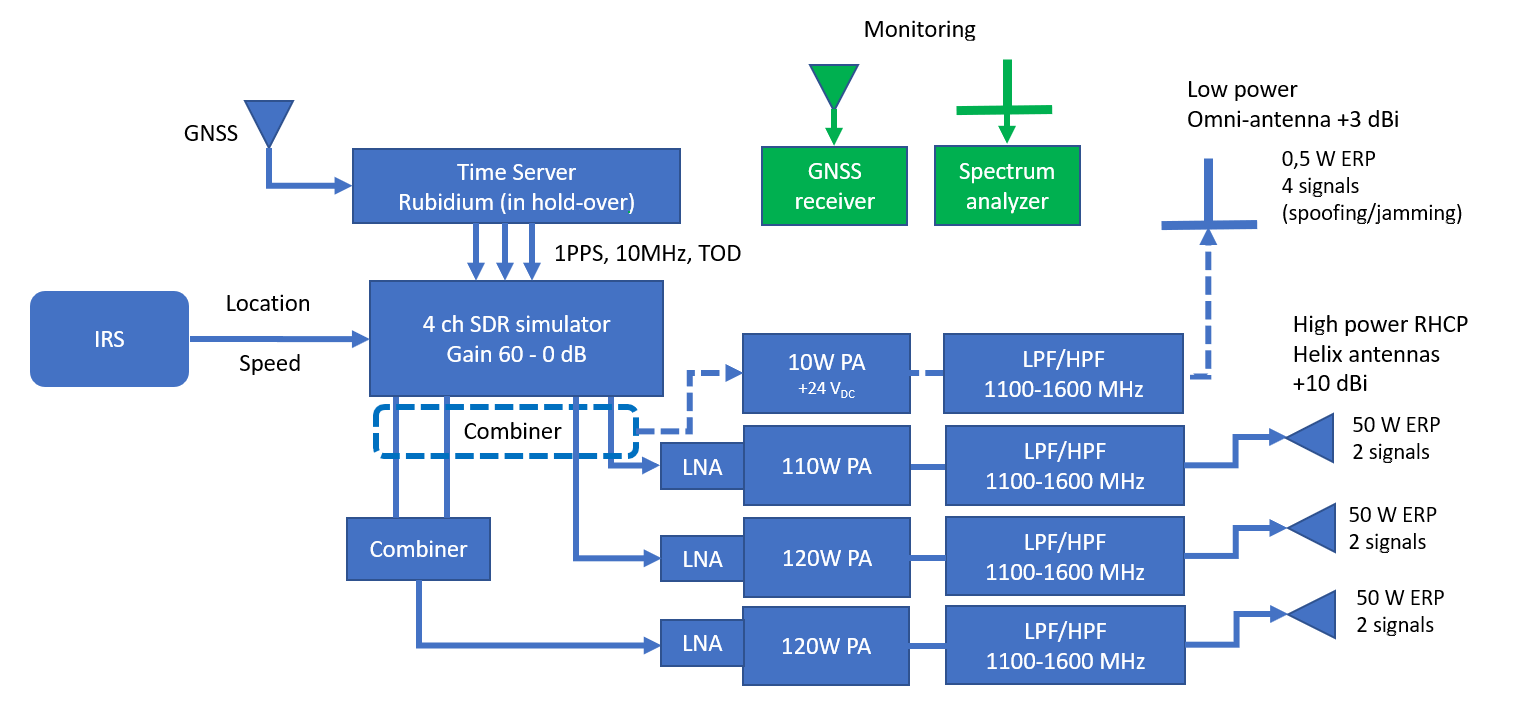
\includegraphics[width=\textwidth]{graphics/appendixG/2025.04.29_M1.1_Winnie-the-spoof.png}
    \caption{Diagram of the mobile jammer}
    \label{fig: M1.1-1 Winnie-the-spoof}
\end{figure}

\subsection{Technical details on the 'ET' meaconing setup 'F5.1'}
The ET system is used to retransmit GNSS signals in the L-band to cause a misdirection of GNSS/GPS receivers. The pickup unit captures the GNSS signals at one location, converts them to an analog optical signal and sends them into an optical fiber to the ET control unit. The pickup unit is located at a great distance from the retransmitter to avoid feedback/looping.
In a rack, the ET control unit is placed together with power amplifiers. The control unit converts the optical signal back to RF, amplifies and filters the GNSS signal. In the control unit, the level can be adjusted and the signal quality assessed with a built-in GNSS receiver. Outputs with different bandwidths can be selected for the current test. The following table gives an overview of the main frequency bands and bandwidths available with the ET system.
\begin{table}[H]
\begin{tabular}{|c|c|c|c|}
\hline
\rowcolor[HTML]{C0C0C0}
\textbf{Frequency range (MHz)} & \textbf{Bandwidth (MHz)} & \textbf{Bands} & \textbf{Notes} \\
\hline
1154--1314 & 161 & L5, G3, E5, E6, L2, G2 & Lower L-Band \\
\hline
1554--1615 & 61 & L1, G1, E1 & Upper L-Band \\
\hline
1210--1243 & 33 & L2 &  \\
\hline
1557--1594 & 37 & L1, E1 &  \\
\hline
1154--1314; 1554--1595 & WB & WB & Wideband (WB) \\
\hline
\end{tabular}
\caption{Overview of the main frequency bands and bandwidths available with the ET system}
\end{table}


%% content ends here
